\section{Transazioni con Protezione della Privacy Integrata}
La privacy fornita in modo nativo da Bitcoin ed Ethereum è limitata alla pseudonimia, mentre i dettagli della transazione non sono riservati. L'importo della transazione ed i beni trasferiti, i loro metadati e le relazioni con altre transazioni possono essere  banalmente verificate da chiunque. In effetti, in questo contesto, esistono tre aspetti della privacy: la privacy del mittente, la privacy del destinatario e la privacy dei dettagli della transazione. Vari metodi crittografici possono essere applicati per affrontarli, come mostrato nella Tabella \ref{table:PrivacyPreservingTechniques}.

\begin{table}[tp]%
	\caption{Tecniche di Conservazione della Privacy per le Blockchain}
	\label{table:PrivacyPreservingTechniques}\centering %
	\begin{tabular}{l|p{2cm}c|p{2.5cm}|p{2cm}}
		\hline
		Tecnica              & Nasconde il Mittente & Nasconde il destinatario & Nasconde l'Importo \\
		\hline
		Stealth Address      & N                    & Y                        & N                  \\
		Pedersen Commitments & N                    & N                        & Y                  \\
		Ring Signatures      & Y                    & N                        & N                  \\
		zk-SNARKs            & Y                    & N                        & Y                  \\
		\hline
	\end{tabular}
\end{table}

IoTeX integra lo stealth address per la privacy del destinatario, la ring signature per la privacy del mittente, ed il Pedersen Commitments per nascondere l'importo della transazione, con le seguenti innovazioni e miglioramenti:

\begin{itemize}
	\item Un algoritmo di stealth address leggero, progettato per sollevare i destinatari dall'onere di scandire l'intera blockchain per venire a conoscenza delle transazioni in arrivo;

	\item Una ring signature ottimizzata per ridurne le dimensioni, senza utilizzare una configurazione distribuita di tipo trusted.
\end{itemize}


\subsection{Nascondere il destinatario della transazione mediante Codice di Pagamento Inoltrabile}

\subsubsection{Stealth Address}
La tecnica dello stealth address nasce dal protocollo Cryptonote \cite{c28}, che risolve il problema del destinatario utilizzando un protocollo di scambio di chiavi Diffie-Hellman a "mezzo giro". Supponendo che \emph{Bob} voglia nascondere il fatto che riceverà dei token da \emph{Alice}, ecco come funzionerebbe:

\begin{enumerate}
	\item \emph{Bob} crea due coppie di chiavi private e pubbliche, indicate come $(a, A)$ e $(b, B)$, dove $A = a\cdot G$, $B = b\cdot G$, e $G$ è il punto base su una curva ellittica.

	\item \emph{Bob} divulga le chiavi pubbliche $(A, B)$, note come il suo "stealth address";

	\item \emph{Alice} calcola e invia i token a $P = H (rA)\cdot G + B$ usando una funzione hash $H$, un numero casuale e grande $r$  e lo stealth address di \emph{Bob} $B$. Questa transazione viene trasmessa insieme a $R = r\cdot G$;
	\item  \emph{Bob} monitora tutte le transazioni, calcola $P' = (H(aR) + b)\cdot G$ (poiché egli conosce $a$, $b$, $R$ e $G$) con la speranza che $P'$ sia uguale a $P$. Se $P' = P$, Bob potrà spendere i token inviati a $P'$ con la chiave privata $H(aR) + b$.
\end{enumerate}

Un inconveniente evidente dello stealth address è che il destinatario deve monitorare tutte le transazioni della rete (il che non è l'ideale nel mondo IoT), oppure in alternativa deve basarsi sull'assistenza di un full-node di fiducia che lo faccia per lui (il che a un certo livello compromette la privacy).

\subsubsection{Codice di pagamento}
Il codice di pagamento è stato ideato per risolvere l'inconveniente di cui sopra relativo allo stealth address, sacrificando in parte la privacy. L'idea è che \emph{Alice} notifichi a \emph{Bob} un codice di pagamento tramite un metodo riservato, e Bob monitori solo le transazioni verso gli indirizzi derivanti da quel codice. Pertanto, questa proposta presenta due flussi: quello della notifica, che rappresenta una configurazione una-tantum tra certe due parti, e quello di invio, che può accadere più volte tra queste due parti.

Supponendo che \emph{Alice} abbia una coppia di chiavi pubblica-privata principali ($mpub_{Alice}, mpri_{Alice}$) dove $mpub_{Alice} = mpri_{Alice}\cdot G$, ed una coppia di chiavi pubblica-privata di portafoglio ($wpub_{Alice}, wpri_{Alice}$) dove $wpub_{Alice} = wpri_{Alice}\cdot G$; che \emph{Bob} abbia una coppia di chiavi pubblica-privata principali $(mpub_{Bob}; mpri_{Bob})$ dove $mpub_{Bob} = mpri_{Bob}\cdot G$, la notifica una tantum funziona come descritto di seguito:

\begin{enumerate}
	\item \emph{Bob} deriva $B_0 = b_0\cdot G = (mpri_{Bob} + Hash(0, seed, metadata))\cdot G$, lo converte in un indirizzo di notifica $\texttt{addr}(B_0)$, lo pubblica e si mette in ascolto su di esso

	\item  \emph{Alice} sceglie un codice $cc$ a caso; $(mpub_{Alice}||cc)$ è il codice di pagamento per \emph{Alice};

	\item  \emph{Alice} calcola un codice segreto condiviso $S = wpri_{Alice}\cdot B_0$ ed invia il codice di  pagamento mascherato $P' = (mpub_{Alice}||cc)\oplus HMAC512(xofS)$ ad $\texttt{addr}(B_0)$;

	\item Alla ricezione, \emph{Bob} ottiene $wpub_{Alice}$ e recupera $S = wpub_{Alice}\cdot b_0$, scopre $P'$ per ottenere $(mpub_{Alice}||cc)$.
\end{enumerate}

Una volta che il flusso di notifica è completo, \emph{Alice} e \emph{Bob} stabiliscono un canale privato unidirezionale per l'invio di token. Il primo invio funziona come descritto di seguito:

\begin{enumerate}
	\item \emph{Alice} deriva un nuovo indirizzo dal suo codice di pagamento (che è già condiviso con \emph{Bob}) da $A_0 = a_0\cdot G = mpub_{Alice} + Hash(0, seed, metadata)\cdot G$;

	\item \emph{Alice} seleziona la successiva chiave pubblica non ancora utilizzata, derivata da $B_0$. Si noti che $B_0$ è la chiave pubblica inutilizzata per il primo round.

	\item \emph{Alice} calcola il nuovo codice segreto condiviso $S_0 = a_0\cdot B_0$ e calcola la chiave pubblica temporanea utilizzata per inviare la transazione per cui si verifica $B'_0 = B_0 + SHA256(S_0)\cdot G$

	\item \emph{Bob} potrebbe derivare $A_0$ in modo non interattivo poiché conosce il codice di pagamento di Alice, e ascolta solo l'indirizzo derivato da $B'_0 = B_0 + SHA256(S_0)\cdot G$ ed $S_0 = A_0\cdot b_0$.

	\item Alla ricezione, \emph{Bob} può spendere i token con la chiave privata $b_0 + SHA256(S_0)$.

\end{enumerate}

I flussi successivi funzionano in maniera analoga.
\emph{Bob} non ha bisogno di monitorare la rete o affidarsi a un full-node per eseguire la scansione di tutte le transazioni. La transazione di notifica fa trapelare l'intenzione di \emph{Alice} di inviare qualcosa a \emph{Bob}, ma l'effettivo "invio di qualcosa" è nascosto a tutti gli altri.

\subsubsection{Codice di Pagamento Inoltrabile}
Per ridurre ulteriormente la perdita di privacy, abbiamo progettato il \emph{codice di pagamento inoltrabile} basandoci sulla proposta originaria del \emph{codice di pagamento} appena descritta. Mentre il flusso di invio rimane lo stesso, abbiamo migliorato il flusso di notifica per consentire ad \emph{Alice} di condividere segretamente il suo codice di pagamento con \emph{Charlie} senza utilizzare la transazione di notifica, assumendo che \emph{Alice} e \emph{Bob} abbiano un canale privato unidirezionale, e \emph{Bob} e \emph{Charlie} abbiano un altro canale privato unidirezionale. Per ottenere ciò, sfruttiamo i contratti Hashed Timelock (HTLC - \emph{Hashed TimeLock Contracts}), i quali richiedono che il destinatario di un pagamento confermi la ricezione di un pagamento prima di una deadline, generando una dimostrazione di pagamento (\emph{proof of payment}) crittografata, oppure rinunci alla possibilità di reclamare il pagamento, restituendolo al mittente.


Supponendo che \emph{Charlie} abbia una coppia di chiavi pubblica-privata $(mpub_{Charlie}, mpri_{Charlie})$ dove $mpub_{Charlie} = mpri_{Charlie}\cdot G$. Il flusso di notifica migliorato funziona come illustrato di seguito:

\begin{enumerate}
	\item \emph{Charlie} deriva $C_0 = c_0\cdot G = (mpri_{Charlie} + Hash(0, seed, metadata))\cdot G$, lo converte in un indirizzo di notifica $\texttt{addr}(C_0)$, lo pubblica. Si noti che $C_0$ è pubblicato per \emph{Alice} al fine calcolare il codice segreto condiviso, ma non per ricevere transazioni;

	\item \emph{Alice} genera il suo codice di pagamento $(mpub_{Alice}||cc)$ nello stesso modo;

	\item \emph{Alice} calcola un codice segreto condiviso $S = wpri_{Alice}\cdot C_0$ e invia il codice di pagamento mascherato $P' = (mpub_{Alice}||cc) \oplus HMAC512(xofS)$ con $X$ token come incentivo e $HTLC(Hash^2(cc))$ a \emph{Bob} usando il loro canale privato unidirezionale, dove $HTLC$, come parte dello script di blocco o riscatto, afferma che i token diventano
	      spendibili se viene fornita la pre-immagine di $Hash^2(v)$, ovvero $Hash (cc)$;

	\item \emph{Bob}, incentivato dai token inviati da Alice, invia $P'$, $Y$, $Y < X$ token ed $HTLC(Hash^2(v))$ a \emph{Charlie} usando il loro canale privato unidirezionale;

	\item \emph{Charlie}, dopo aver ricevuto la transazione di \emph{Bob}, calcola $S = wpub_{Alice}\cdot c_0$ per scoprire il codice di pagamento di \emph{Alice}, e spendere la transazione rivelando $Hash(cc)$, che rende spendibile la transazione da \emph{Alice} a \emph{Bob}, e che premia \emph{Bob}.
\end{enumerate}

Una volta che questo flusso viene completato, \emph{Alice} e \emph{Charlie} stabiliscono un canale privato unidirezionale per l'invio di token. È interessante notare che il tragitto della transazione di \emph{Alice} potrebbe consistere di più salti.

I nostri codici di pagamento inoltrabili offrono una privacy maggiore in termini di occultamento dell'intenzione di "inviare qualcosa" sulla blockchain, sfruttando i canali privati esistenti, e senza aggiungere alcun overhead di elaborazione o di archiviazione per i nodi. Inoltre, sebbene progettati per scenari IoT, i codici di pagamento inoltrabili risultano utilizzabili per la maggior parte delle blockchain come Bitcoin.

\subsection{Abilitare Transazioni Riservate}

\subsubsection{Definizione del Problema}
In Figura \ref{fig:fig4} viene mostrata una tipica transazione sulla blockchain Bitcoin. In sostanza, una transazione blockchain è semplicemente una tupla $({pk_{in,i}, {pk_{out,j},{v_{i,j}}}})$, dove $({pk_{in,i}})$ rappresentano indirizzi di input, ${pk_{out,j}}$ indirizzi di output, e ${v_{i,j}}$ sono gli importi delle transazioni tra gli indirizzi di input e output. Poiché le transazioni Bitcoin sono memorizzate in chiaro in un registro pubblico, ciò ha sollevato molti problemi in termini di sicurezza e privacy.

\begin{figure}[ht]
	\centering
	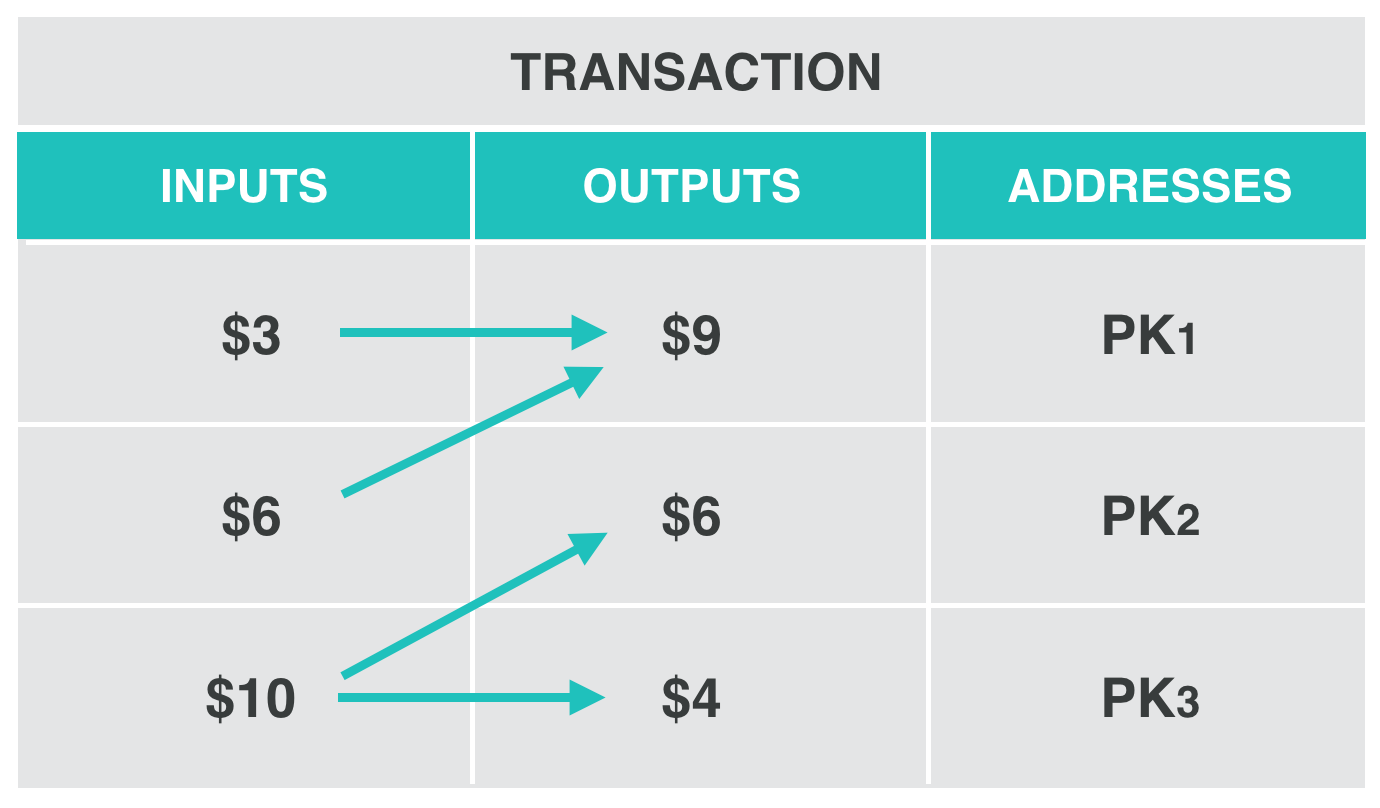
\includegraphics[width=0.5\textwidth]{Figura4.png}
	\caption{Una transazione sulla Blockchain Bitcoin}
	\label{fig:fig4}
\end{figure}

L'obiettivo delle transazioni riservate (vedere la Figura \ref{fig:fig5}) è quello di consentire solo ai mittenti e ai destinatari delle transazioni di rivelarne il valore ${v_{i,j}}$ e di nasconderlo al resto del mondo. Inoltre, le transazioni riservate consentono comunque alle altre entità della rete di verificare la validità di tali transazioni, pur senza poter vedere gli importi effettivi. La realizzazione di transazioni riservate su blockchain richiede un certo numero di tecniche crittografiche avanzate.

\begin{figure}[ht]
	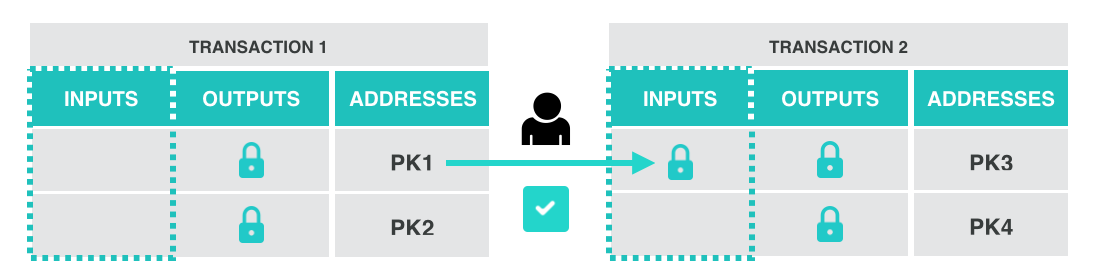
\includegraphics[width=\textwidth]{Figura5.png}
	\label{fig:fig5}
	\caption{Una transazione Riservata Con Verificabilità Pubblica}
\end{figure}

\subsubsection{Prova di Conoscenza}
Una prova di conoscenza (\emph{proof of knowledge}), indicata con $(P, V)$, è una dimostrazione interattiva tra un dimostratore $P$ ed un verificatore $V$, in cui il dimostratore vuole dimostrare di conoscere alcune informazioni. In particolare, $P$ possiede $(x, w)$ legati da una relazione $R$, dove $x$ è il problema e $w$ è la soluzione (anche detta \emph{testimone}). $V$ conosce $x$, e confermerà solo se $P$ riesce a convincere $V$ che egli conosce $w$.

\subsubsection{Dimostrazione a conoscenza zero}
In un protocollo a conoscenza zero (\emph{zero-knowledge}), il dimostratore dimostra un'affermazione al verificatore, senza rivelare nient'altro sull'affermazione oltre alla veridicità della stessa, cosa che protegge il dimostratore da verificatori malevoli che cerchino di acquisire più informazioni del necessario. Il protocollo può essere \emph{interattivo} o \emph{non interattivo}. La differenza chiave delle dimostrazioni non interattive è che tutte le interazioni consistono in un singolo messaggio inviato dal dimostratore al verificatore. Usiamo la notazione $\texttt{NIZKPoK}(\alpha, \beta): a = g^{\alpha} \wedge b = g^{\beta}$ per denotare una prova a conoscenza zero dei valori $\alpha$ e $\beta$ non interattiva, tale che $a = g^{\alpha} e b = g^{\beta}$. Si presume che tutti i valori non racchiusi tra parentesi siano noti al verificatore. Quando usiamo una dimostrazione a conoscenza zero non interattiva per autenticare dati ausiliari, lo schema risultante è indicato come \emph{firma di conoscenza} ("\emph{Signature of Knowledge}")\cite{c8}. Fondamentalmente, uno schema a firma di conoscenza significa che un soggetto in possesso di una soluzione $w$ al problema $x$ ha firmato il messaggio $m$. Per il \texttt{NIZKPoK} di cui sopra, usiamo la notazione $\texttt{SoK}[m](\alpha, \beta): a = g^{\alpha} \wedge b = g^{\beta}$ per indicare una firma di conoscenza sul messaggio $m$.

\subsubsection{Ring Signature}
Il concetto di firma ad anello (\emph{"Ring Signature"}) è stato introdotto per la prima volta da Rivest et al. \cite{c27} nel 2001 come un tipo particolare di firma di gruppo. In una firma ad anello, il firmatario del messaggio seleziona un insieme di membri dell'anello, compreso se stesso, come possibili firmatari di messaggi. Il verificatore può essere convinto che la firma sia stata effettivamente generata da uno dei membri dell'anello.
Tuttavia, il verificatore non è in grado di stabilire quale membro abbia effettivamente generato la firma. A differenza di una firma di gruppo generica, uno schema di firma ad anello non comporta la scelta di un manager del gruppo per la gestione dell'insieme dei membri dell'anello, eliminando in tal modo la possibilità che l'identità del vero firmatario del messaggio possa essere rivelata dal manager del gruppo. Al fine di garantire l'anonimato nelle transazioni di token mediante smart contract, nella criptovaluta Monero è stato utilizzato un tipo speciale di firma ad anello, la cosiddetta firma ad anello collegabile \cite{c20}. La firma ad anello collegabile ha la proprietà aggiuntiva per cui qualunque firma generata dallo stesso firmatario, sia che firmi lo stesso messaggio o messaggi diversi, ha un identificatore (chiamato tag) che collega le firme. Questa proprietà consente a terzi di verificare in modo efficiente che le firme sono state generate dallo stesso soggetto, senza divulgarne l'identità. La firma ad anello collegabile utilizzata in Monero viene chiamata  Multi-Layered Linkable Spontaneous Anonymous Group Signature (MLSAG)\cite{c22}, che è una firma ad anello su un insieme di vettori di chiavi ed ha una complessità di comunicazione di $O(m(n + 1))$, dove $m$ è il numero di coppie di chiavi pubbliche/private di proprietà del firmatario ed $n$ è la dimensione dell'anello.

\subsubsection{Accumulatore}
Gli accumulatori unidirezionali, che furono proposti per la prima volta da Benaloh e de Mare in \cite{c2}, sono definiti come funzioni hash unidirezionali con la proprietà di essere \emph{quasi-commutative}. Una funzione quasi-commutativa $f: X \times Y \Rightarrow X$ è tale che, per ogni $x \in X$ e per ogni $y_1, y_2 \in Y$, abbiamo che $f(f(x, y_1), y_2) = f(f(x, y_2), y_1)$. Un accumulatore unidirezionale ci consente di combinare un insieme di valori in una raccolta sicura e questa raccolta non dipende dall'ordine in cui i valori vengono accumulati. Può anche essere usato per generare un testimone, ciò consente a un soggetto di attestare che un determinato valore fa effettivamente parte dell'accumulatore.

\subsubsection{Schema di Impegno}
Uno schema di impegno (\emph{"commitment scheme"}) è un protocollo che consente a un utente di impegnarsi per un certo valore a sua scelta, senza rivelare tale valore al destinatario dell'impegno. In un secondo momento, quando all'utente viene chiesto di rivelare il valore impegnato, il destinatario avrà i mezzi per verificare che il valore rivelato sia realmente legato al suo impegno in modo incondizionato. Uno schema di impegno dovrebbe soddisfare due requisiti. Mentre il requisito di \emph{occultamento} impedisce al destinatario di apprendere il contenuto dell'impegno,
il requisito di \emph{vincolo} impedisce al mittente di barare nel momento in cui rivela l'impegno. Nello schema di impegno di Pedersen \cite{c23}, i parametri di dominio sono un gruppo ciclico $\mathds{G}$ di primo ordine $q$, e generatori $(g_0,..., g_m)$. Per impegnarsi per i valori $(v_1,..., v_m) \in \mathds{Z}^m_q$, un soggetto sceglie un numero casuale $r \in \mathds{Z}_q$ e imposta l'impegno
$C = \texttt{PedCom}(v_1,..., v_m; r) = g^r_0\prod^m_{i=1}g^{v_i}_i$.


\subsubsection{I nostri miglioramenti}
In \cite{c31}, Sun et al. hanno presentato il RingCT 2.0, che utilizzava un accumulatore crittografico per ridurre ulteriormente la complessità della comunicazione a $O(n)$ al prezzo di calcoli aggiuntivi. Notiamo che, sebbene RingCT 2.0 abbia ridotto la complessità della comunicazione in modo significativo rispetto a MLSAG, la generazione dei parametri di dominio dell'accumulatore richiede un processo di "configurazione fidata" una tantum come avviene in Zcash. Quindi un soggetto deve avere fiducia che chiunque abbia generato i parametri segreti li distrugga poi quando ha finito, cosa che ha sollevato problemi di sicurezza e privacy per il sistema. Per risolvere
questo problema, la nostra soluzione è quella di utilizzare un protocollo di calcolo multi-parte sicuro (SMPC) tra una serie di nodi di avvio della blockchain, per generare parametri di dominio segreti in modo sicuro e distribuito. Inoltre, i seguenti settori sono attualmente in fase di studio per migliorare i protocolli simil-RingCT in termini di overhead computazionale e di comunicazione:

\begin{itemize}
	\item Un nuovo schema di firma ad anello collegabile con complessità di comunicazione inferiore a $O(n)$
	\item Un nuovo approccio per l'aggregazione di più firme ad anello collegabili
	\item Un protocollo sigma per la configurazione affidabile dei parametri segreti del dominio
\end{itemize}

Il nostro obiettivo è proporre una nuova soluzione per le transazioni riservate che sia in grado di raggiungere un buon compromesso tra comunicazione e costo computazionale.

\subsection{Dimostrare l'intervallo dell'importo della transazione mediante Bulletproofs}
Come alternativa agli Impegni di Pedersen, di recente è stato proposto Bulletproofs \cite{c5}, un nuovo protocollo non interattivo con dimostrazione a conoscenza zero, con prove molto brevi e senza configurazione trusted, che riduce la dimensione dell'intervallo di prova da lineare a sublineare e riduce ulteriormente la dimensione della transazione senza costi aggiuntivi in termini di calcolo. Dal momento che  Bulletproofs si adatta bene al nostro principio di progettazione, esso sarà integrato in IoTeX.
